\documentclass[UTF8,a4paper,12pt,fontset=none]{ctexart}
\setCJKmainfont{SimSun}
\setCJKsansfont{SimHei}
\setCJKmonofont{FangSong}
\newCJKfontfamily\heiti{SimHei}
\newCJKfontfamily\kaiti{KaiTi}
\newCJKfontfamily\fangsong{FangSong}
\newCJKfontfamily\songti{SimSun}

\usepackage{geometry}
\usepackage{graphicx}
\usepackage{booktabs}
\usepackage{longtable}
\usepackage{array}
\usepackage{float}
\usepackage{amsmath}
\usepackage{amssymb}
\usepackage{hyperref}
\usepackage{caption}
\usepackage{subcaption}
\usepackage[numbers,sort&compress]{natbib}
\usepackage{enumitem}
\usepackage{xcolor}
\usepackage{fancyhdr}
\usepackage{titlesec}
\usepackage{titling}
\usepackage{etoolbox}
\usepackage{indentfirst}
\makeatletter
\def\tagform@#1{\maketag@@@{\hspace{0.5em}公式(\ignorespaces#1\unskip\@@italiccorr)\hspace{0.5em}}}
\renewcommand{\eqref}[1]{公式\textup{(\ref{#1})}}
\makeatother
\usepackage{tocloft}

\geometry{left=3.17cm,right=3.17cm,top=2.54cm,bottom=2.54cm}
\hypersetup{colorlinks=true, linkcolor=black, citecolor=black, urlcolor=black}
\graphicspath{{figures/}}

\newcommand{\papertitle}{大国博弈下中国半导体相关产品\\进口来源结构演化与供应链风险评估研究}
\newcommand{\school}{最终提交前由参赛队填写}
\newcommand{\teamname}{最终提交前由参赛队填写}
\newcommand{\members}{最终提交前由参赛队填写}
\newcommand{\advisor}{最终提交前由参赛队填写}

\setlength{\parindent}{2em}
\setlength{\parskip}{0pt}
\linespread{1.667}\selectfont
\setlist{nosep,leftmargin=2em}
\captionsetup{font=normalsize,labelfont=bf,labelsep=quad}
\captionsetup[table]{position=top}
\AtBeginEnvironment{tabular}{\fontsize{10.5}{12}\selectfont}
\AtBeginEnvironment{longtable}{\fontsize{10.5}{12}\selectfont}
\AtBeginEnvironment{table}{\fontsize{10.5}{12}\selectfont}
\setlength{\floatsep}{8pt plus 2pt minus 2pt}
\setlength{\textfloatsep}{10pt plus 2pt minus 2pt}
\setlength{\intextsep}{8pt plus 2pt minus 2pt}
\setlength{\headheight}{14pt}

\renewcommand\thesection{\chinese{section}}
\renewcommand\thesubsection{（\chinese{subsection}）}
\renewcommand\thesubsubsection{\arabic{subsubsection}.}

\titleformat{\section}{\heiti\zihao{-3}}{\thesection、}{0pt}{}
\titleformat{\subsection}{\kaiti\zihao{4}}{\thesubsection}{0pt}{}
\titleformat{\subsubsection}{\songti\zihao{-4}\bfseries}{\thesubsubsection}{0.5em}{}
\titlespacing*{\section}{0pt}{12pt}{0pt}
\titlespacing*{\subsection}{0pt}{0pt}{0pt}
\titlespacing*{\subsubsection}{0pt}{0pt}{0pt}

\ctexset{
  contentsname = {目\quad 录},
}

\pagestyle{fancy}
\fancyhf{}
\fancyfoot[C]{\zihao{5}\thepage}
\renewcommand{\headrulewidth}{0pt}

\newcommand{\paperabstract}[2]{%
  \clearpage
  \begin{center}
  {\heiti\zihao{4} 摘\quad 要}
  \end{center}
  \hspace{2em}#1
  \vspace{0.8ex}

  {\heiti\zihao{-4} 关键词：}#2
}

\setcounter{tocdepth}{2}
\renewcommand{\cftsecfont}{\heiti\bfseries}
\renewcommand{\refname}{\heiti\zihao{4} 参考文献}

\begin{document}

% ============ 封面页 ============
\begin{titlepage}
\begin{center}
  {\heiti\zihao{3} 作品编号：\underline{\hspace{4cm}}}\\[2.5cm]
  {\zihao{2} 2026年（第十二届）全国大学生统计建模大赛}\\[0.8cm]
  {\zihao{-1} 参\quad 赛\quad 作\quad 品}\\[2.5cm]
  {\fangsong\zihao{-2}
  \renewcommand{\arraystretch}{1.5}
  \begin{tabular}{r@{\hspace{0.5em}：\hspace{0.5em}}l}
    参赛学校 & \school \\
    论文题目 & \papertitle \\
    参赛队员 & \members \\
    指导老师 & \advisor \\
  \end{tabular}}
\end{center}
\end{titlepage}

% ============ 摘要 ============
\paperabstract{%
在大国科技竞争和出口管制持续强化的背景下，半导体相关产品进口来源结构已成为评估产业链供应链安全的重要切入点。本文基于 CEPII BACI HS07 数据库 \citep{cepii_baci}，构建 2008--2024 年中国自全球进口四类半导体相关 HS6 产品的出口国--产品--年份平衡面板数据，从描述统计、风险指数和统计检验三个层次考察政策冲击下的进口来源结构演化。研究首先从进口规模、美国份额、主要来源国和 HHI 集中度四个角度刻画结构变化事实；其次构建半导体进口供应链风险指数 SIRI，将来源集中、政策暴露、替代不足和结构波动纳入统一评分框架，按产品--年份计算 0--100 综合风险分值；最后结合 OLS 固定效应回归（进口额）和 PPML 估计（进口份额）以及多项稳健性检验，讨论政策节点下的统计证据边界。结果显示，2017--2024 年间，半导体制造设备（848620）的美国进口份额从 27.92\% 降至 9.88\%，处理器及控制器（854231）和存储器（854232）同样下降，但其他电子集成电路（854239）方向相反。2024 年 SIRI 排序显示，854239 和 854232 的综合风险相对更高，主要驱动因素是来源集中和替代不足而非政策暴露——提示高对美依赖不等于高综合风险。统计检验揭示了一个层次化的管制传导过程：2018 年实体清单扩容后美国来源绝对进口额显著上升（$p=0.002$），但份额未显著下降，反映了企业的"恐慌性囤货"行为；2022--2023 年出口管制新规成为转折点，PPML 估计显示美国来源份额下降约 25--27\%（$p<0.001$），绝对进口额于 2023 年开始显著相对下滑。产品层面异质性显著：处理器类产品 2018 年后进口额先升后降，存储器类产品 2018 年后即大幅下降，其他集成电路类产品则持续上升。进一步地，本文在未接入 GDELT 的 BACI-only 设定下，将产品池扩展至 20 个半导体相关 HS6 编码，构造年度进口来源网络，并进行下一年 SIRI 风险预测的原型验证。本文为关键半导体产品进口安全监测提供了可解释、可复现的统计建模框架，并讨论了结论的适用范围与局限。
}{大国博弈；半导体；进口来源结构；供应链风险；统计建模}


% ============ 目录 ============
\clearpage
\begin{center}
{\heiti\zihao{4} 目\quad 录}
\end{center}
\begingroup
\renewcommand{\contentsname}{}
\tableofcontents
\endgroup

% ============ 表格与插图清单 ============
\clearpage
\begin{center}
{\heiti\zihao{4} 表格与插图清单}
\end{center}
\begingroup
\renewcommand{\listtablename}{\heiti\zihao{4}\bfseries 表格}
\renewcommand{\listfigurename}{\heiti\zihao{4}\bfseries 插图}
\listoftables
\listoffigures
\endgroup
\clearpage

% ============ 正文（页码从1开始） ============
\setcounter{page}{1}
\begin{center}
{\zihao{3} \papertitle}
\end{center}
\vspace{0.5cm}
\section{研究背景与问题提出}

半导体是数字经济、先进制造和国家经济安全的重要基础。近年来，围绕先进计算、半导体制造设备和关键集成电路的出口管制不断加强，全球半导体贸易网络面临更强的政策不确定性 \citep{us_bis_controls}。对中国而言，进口来源是否集中、关键来源是否发生替代、不同产品风险是否一致，直接关系到产业链供应链韧性评估。

已有讨论常将半导体供应链风险概括为单一方向的“脱钩”或“断链”，但从统计建模角度看，贸易结构变化可能同时受到出口管制、全球产业周期、中国需求扩张和第三方产能调整影响。因此，本文不把美国出口管制视为唯一解释变量，而是将其作为重要政策背景，重点研究中国半导体相关产品进口来源结构的演化事实和风险暴露。

本文围绕三个问题展开：第一，2018 年以来，中国半导体相关产品进口来源结构是否发生明显变化；第二，不同产品的来源替代路径和风险暴露是否存在差异；第三，能否构建一个可解释、可复现的进口供应链风险评价指标，为后续政策监测提供量化依据。

本文的贡献主要体现在三点。其一，从单一产品扩展到设备类和集成电路类四个 HS6 产品，避免用单一产品概括整个半导体贸易结构。其二，构建 SIRI 风险指数，把来源集中、政策暴露、替代不足和结构波动纳入统一框架。其三，在固定效应回归不显著的情况下，明确区分描述性结构变化和严格因果识别，保持结论边界清楚。

\section{文献综述与理论基础}

\subsection{供应链风险测度研究}

供应链风险研究通常强调风险并非只来自单一断供事件，而是来自需求波动、供应中断、政策限制、物流受阻和关键节点失效等多类冲击的叠加 \citep{chopra2004managing,juttner2005supply}。对进口依赖型产业而言，风险暴露不仅表现为某一来源国份额较高，也体现为供应商结构过度集中、替代来源不足以及来源结构在短期内剧烈波动。因而，供应链安全评估需要同时观察脆弱性和恢复能力：前者对应冲击发生时受影响的可能程度，后者对应通过多元来源和替代路径恢复供给的能力。

这一视角为本文 SIRI 指数提供理论基础。本文不把半导体进口风险简化为“美国份额”单一指标，而是将来源集中、政策暴露、替代不足和结构波动同时纳入评价。这样的设定有助于识别两类容易被忽略的情形：一是对美份额不高但非美来源高度集中的结构性风险，二是总进口规模稳定但来源替代能力不足导致的隐性脆弱性。

\subsection{半导体贸易与出口管制研究}

半导体产业具有高度全球分工特征，设计、制造、设备、材料、封装测试和终端需求分布在不同经济体之间。全球价值链研究指出，信息技术降低了跨境协调成本，使生产环节更容易在国家间分解和重组 \citep{baldwin2016great}。因此，半导体贸易结构不能只看总体进口额，更需要在产品级层面区分制造设备、存储器、处理器及其他集成电路等类别，因为不同产品对应的来源国组合、技术约束和替代空间并不相同。

近年来，美国针对先进计算芯片、半导体制造设备和相关技术的出口管制构成了本文的重要政策背景 \citep{us_bis_controls}。但从贸易数据解释角度看，进口来源变化可能同时受到出口管制、全球半导体周期、中国需求结构、第三方产能扩张和企业库存调整等因素影响。因此，本文将出口管制作为观察结构演化的关键时间背景，而不直接把产品级贸易份额变化表述为单一政策冲击的因果结果。

\subsection{贸易网络与风险预测研究}

网络视角能够把贸易关系从双边份额扩展为节点、边和权重共同构成的结构对象。社会与经济网络理论表明，节点中心性、连接密度和替代路径会影响冲击传播和系统韧性 \citep{jackson2010social}。用于中国半导体相关产品进口研究时，年度贸易网络可以同时刻画来源集中度、主要来源国更替、非美替代路径以及某一关键来源受限时的潜在传播影响。

在预测层面，图表示学习为利用网络结构生成预测输入提供了技术工具，例如 GraphSAGE 将节点邻域信息聚合为可用于下游任务的表示 \citep{hamilton2017inductive}。但这类方法在本文中只构成预测扩展的输入视角，不能替代因果识别。也就是说，贸易网络特征可以用于探索下一年 SIRI 风险是否具有可预测性，但不能据此断言某一政策事件造成了特定贸易结构变化。

\subsection{文献评述与本文定位}

综合来看，既有研究为供应链风险来源、全球价值链分工和网络结构分析提供了基础，但直接服务于本文问题时仍有三点需要补足：第一，半导体相关产品内部差异明显，使用总体贸易额容易掩盖设备类和集成电路类产品的风险来源差异；第二，单一来源国份额难以同时反映集中、替代不足和结构波动；第三，预测模型若缺少明确证据边界，容易把相关性或预测性能误写成政策因果效应。

据此，本文定位为产品级 BACI 数据驱动的进口来源结构研究：先基于 HS6 产品--年份面板刻画中国半导体相关产品进口来源演化，再构建可解释的 SIRI 风险指数衡量来源集中、政策暴露、替代不足和结构波动，随后用固定效应回归给出谨慎的统计证据边界，最后开展 BACI-only 贸易网络下一年 SIRI 预测扩展。该定位强调可复现的数据链条和可解释的风险评价，同时明确预测扩展不替代前文的描述统计与回归检验。

\section{数据来源与变量构造}

\subsection{数据来源与样本范围}

本文使用 CEPII BACI HS07 年度双边贸易数据 \citep{cepii_baci}，样本期为 2008--2024 年，进口国固定为中国。BACI 数据以 HS6 产品和双边贸易流为基本单位，适合从来源国、产品和年份三个维度刻画中国关键产品进口结构。本文保留年度口径，是为了保证 2008--2024 年样本期内不同产品和来源国之间具有可比性。

\subsection{产品选择与样本构造}

研究对象为四类半导体相关 HS6 产品，具体见表 \ref{tab:products}。这些产品覆盖半导体制造设备、处理器及控制器、存储器和其他电子集成电路，能够同时反映设备类与集成电路类产品的差异。

\begin{table}[H]
\centering
\caption{研究产品范围}
\label{tab:products}
\begin{tabular}{lll}
\toprule
HS6编码 & 产品类别 & 产品含义 \\
\midrule
848620 & 设备类 & 半导体器件或集成电路制造设备 \\
854231 & 集成电路类 & 处理器及控制器 \\
854232 & 集成电路类 & 存储器 \\
854239 & 集成电路类 & 其他电子集成电路 \\
\bottomrule
\end{tabular}
\end{table}


观察单元为出口国--产品--年份。对每个产品，本文保留样本期内曾向中国出口该产品的出口国，并补齐 2008--2024 年的年份维度；未出现的出口国--产品--年份贸易流按 0 处理。处理后的多产品平衡面板共 10608 行，其中正向贸易记录 5619 行，涵盖四个产品的所有历史出口国。

\subsection{变量定义与模型设定}

核心变量包括两类被解释变量：进口额对数 $\ln(Import_{i,p,t}+1)$ 用于衡量贸易规模变化，进口份额 $Share_{i,p,t}$ 用于反映来源国相对地位变化。核心解释变量为美国来源虚拟变量 $US_i$ 与三个政策节点虚拟变量（$Post2018_t$、$Post2022_t$、$Post2023_t$）的交互项，分别捕捉 2018 年实体清单扩容、2022 年出口管制新规和 2023 年持续收紧三个政策阶段对美国来源进口的相对影响。

控制变量包括出口国固定效应（吸收不随时间变化的国别特征）、产品固定效应（吸收产品层面的结构性差异）和年份固定效应（吸收宏观经济周期和全球半导体需求波动）。所有回归使用 HC1 异方差稳健标准误。

\section{描述性统计与来源结构演化}

表 \ref{tab:descriptive} 给出多产品面板的基本描述统计。四类产品均覆盖 17 个年份，但出口国数量和贸易规模存在明显差异。854231、854232 和 854239 的出口国数量高于 848620，说明集成电路类产品的全球贸易来源更广；但更广的来源并不必然意味着风险更低，因为部分产品仍可能集中于少数核心生产网络节点。

\begin{table}[H]
\centering
\scriptsize
\caption{多产品面板描述统计}
\label{tab:descriptive}
\begin{tabular}{lrrrrr}
\toprule
指标 & 全部产品 & 848620 & 854231 & 854232 & 854239 \\
\midrule
观测值 & 10608 & 1020 & 3366 & 2737 & 3485 \\
正向贸易记录 & 5619 & 585 & 1789 & 1251 & 1994 \\
出口国-产品组合 & 624 & 60 & 198 & 161 & 205 \\
年份数 & 17 & 17 & 17 & 17 & 17 \\
平均进口额（千美元） & 246456.38 & 172161.32 & 321346.33 & 261591.24 & 183982.15 \\
平均进口份额 & 0.006410 & 0.016667 & 0.005051 & 0.006211 & 0.004878 \\
\bottomrule
\end{tabular}
\end{table}


图 \ref{fig:total-imports} 展示四类产品的总进口规模变化。不同产品的规模波动差异较大，说明中国半导体相关进口不仅受政策因素影响，也与产业周期和国内需求变化有关。

\begin{figure}[H]
    \centering
    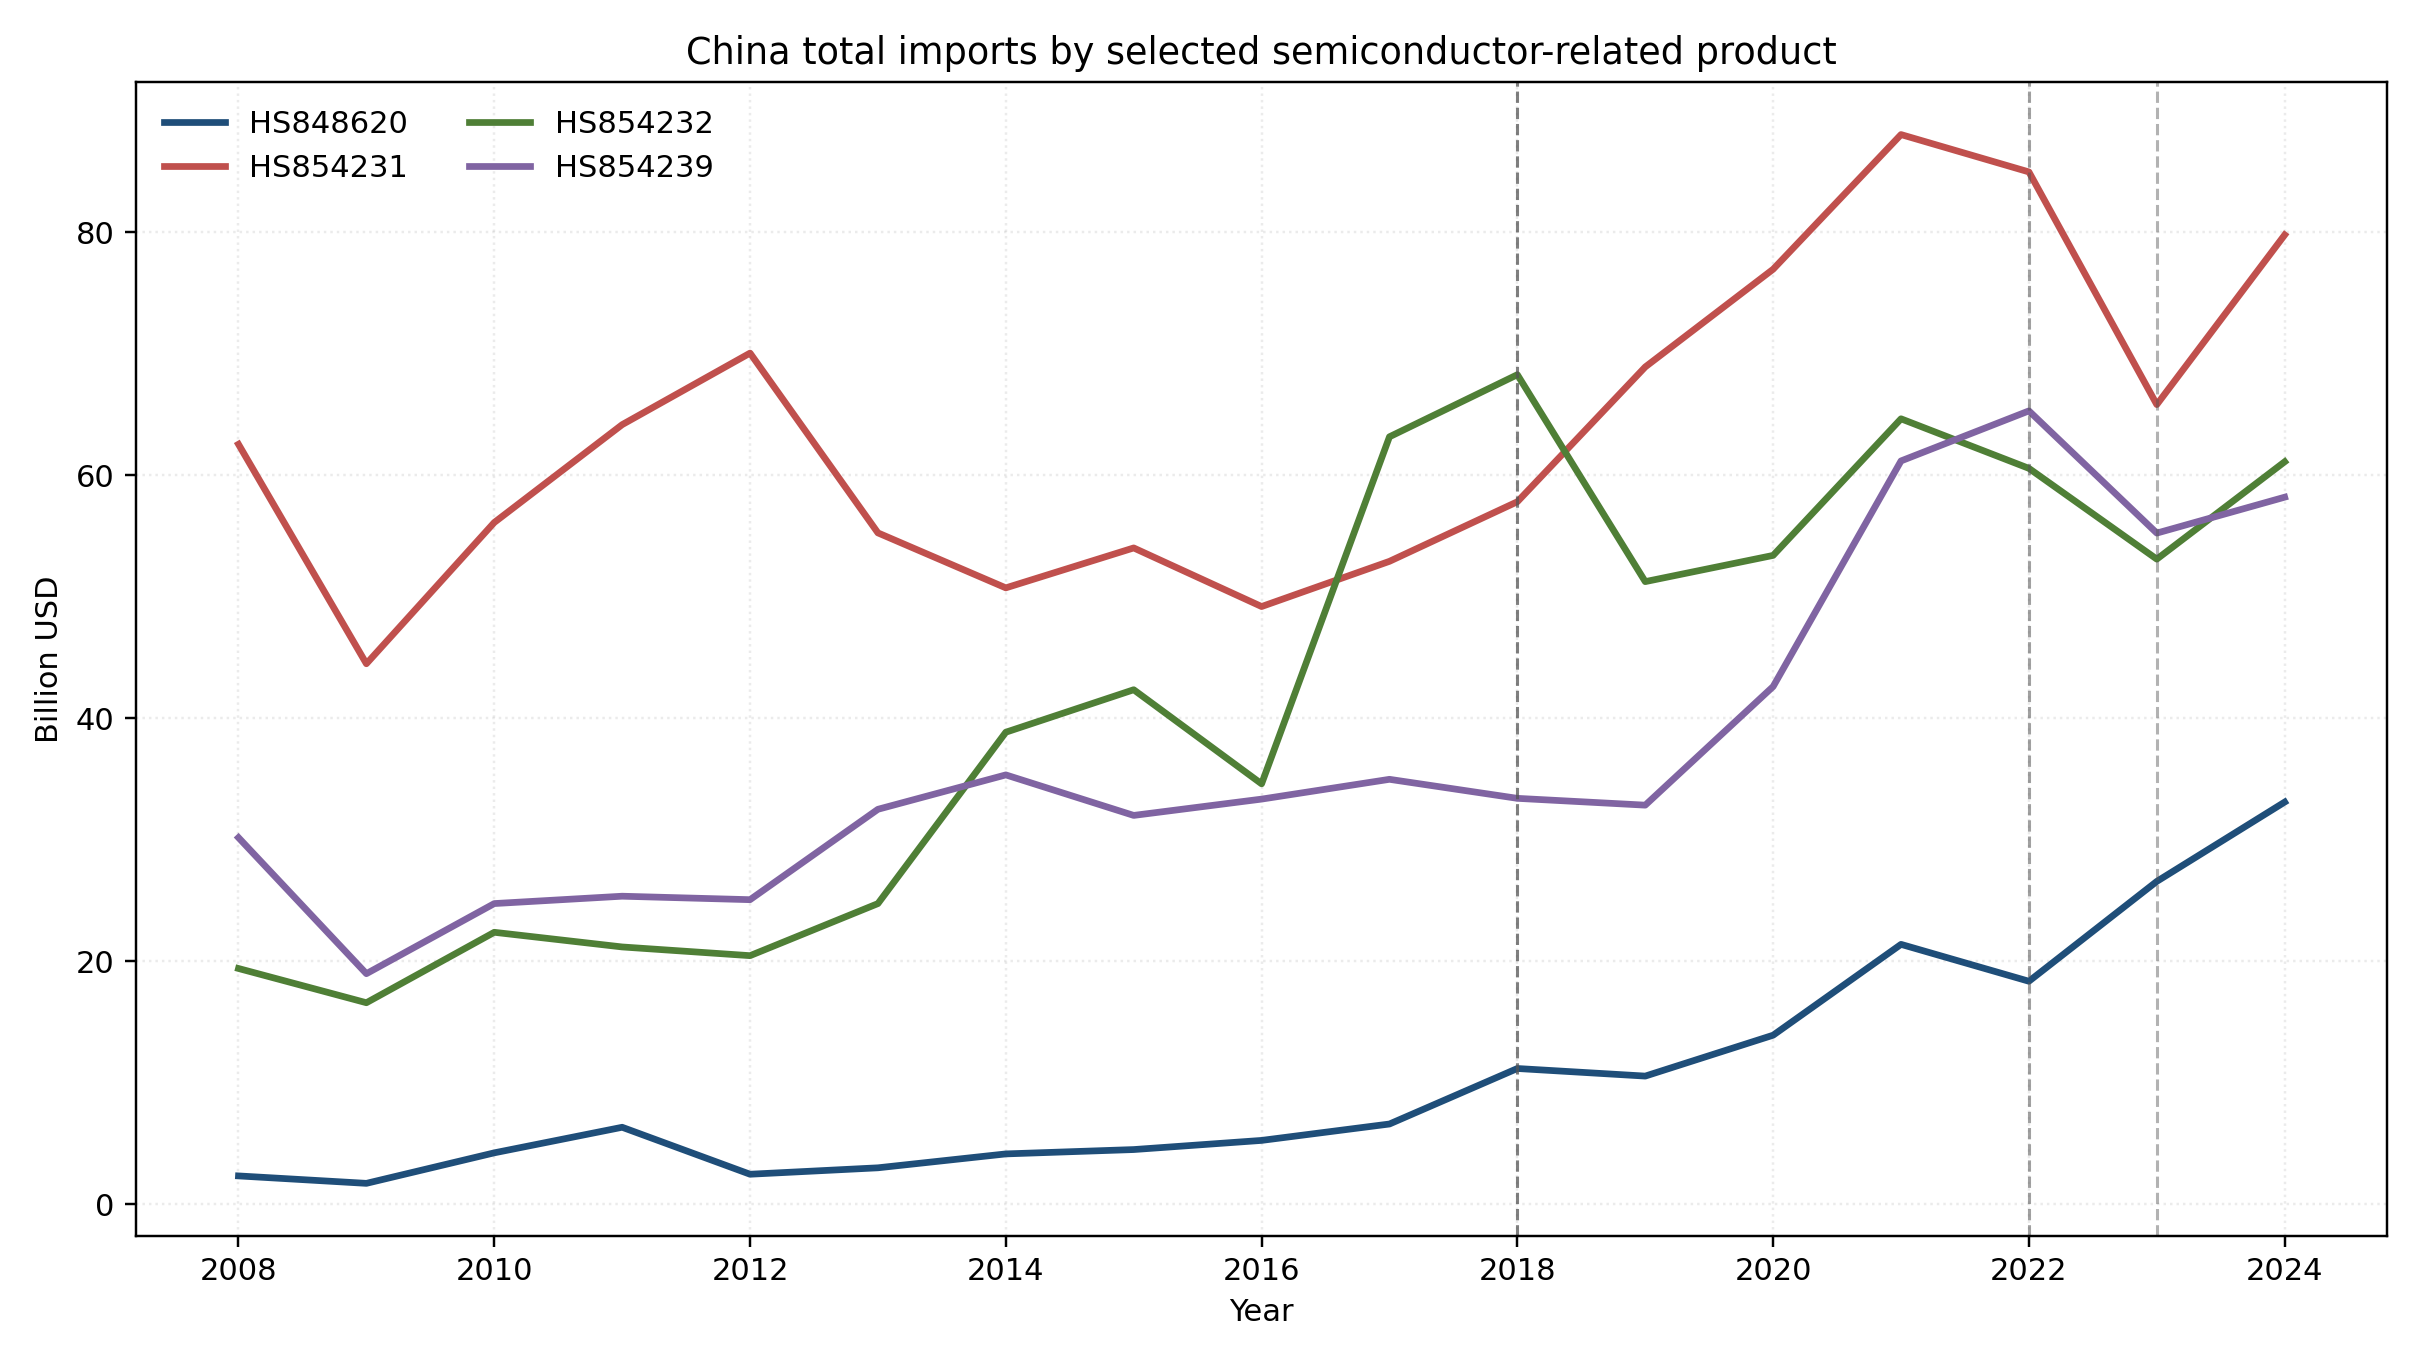
\includegraphics[width=0.92\textwidth]{total_imports_by_product_v02.png}
    \caption{中国半导体相关产品总进口额变化}
    \label{fig:total-imports}
\end{figure}

从美国进口份额看，848620 的美国份额从 2017 年 27.92\% 降至 2024 年 9.88\%，854231 从 12.47\% 降至 9.72\%，854232 从 0.95\% 降至 0.14\%。854239 则从 2.82\% 升至 3.94\%，表明集成电路类产品并非完全同向变化。

\begin{figure}[H]
    \centering
    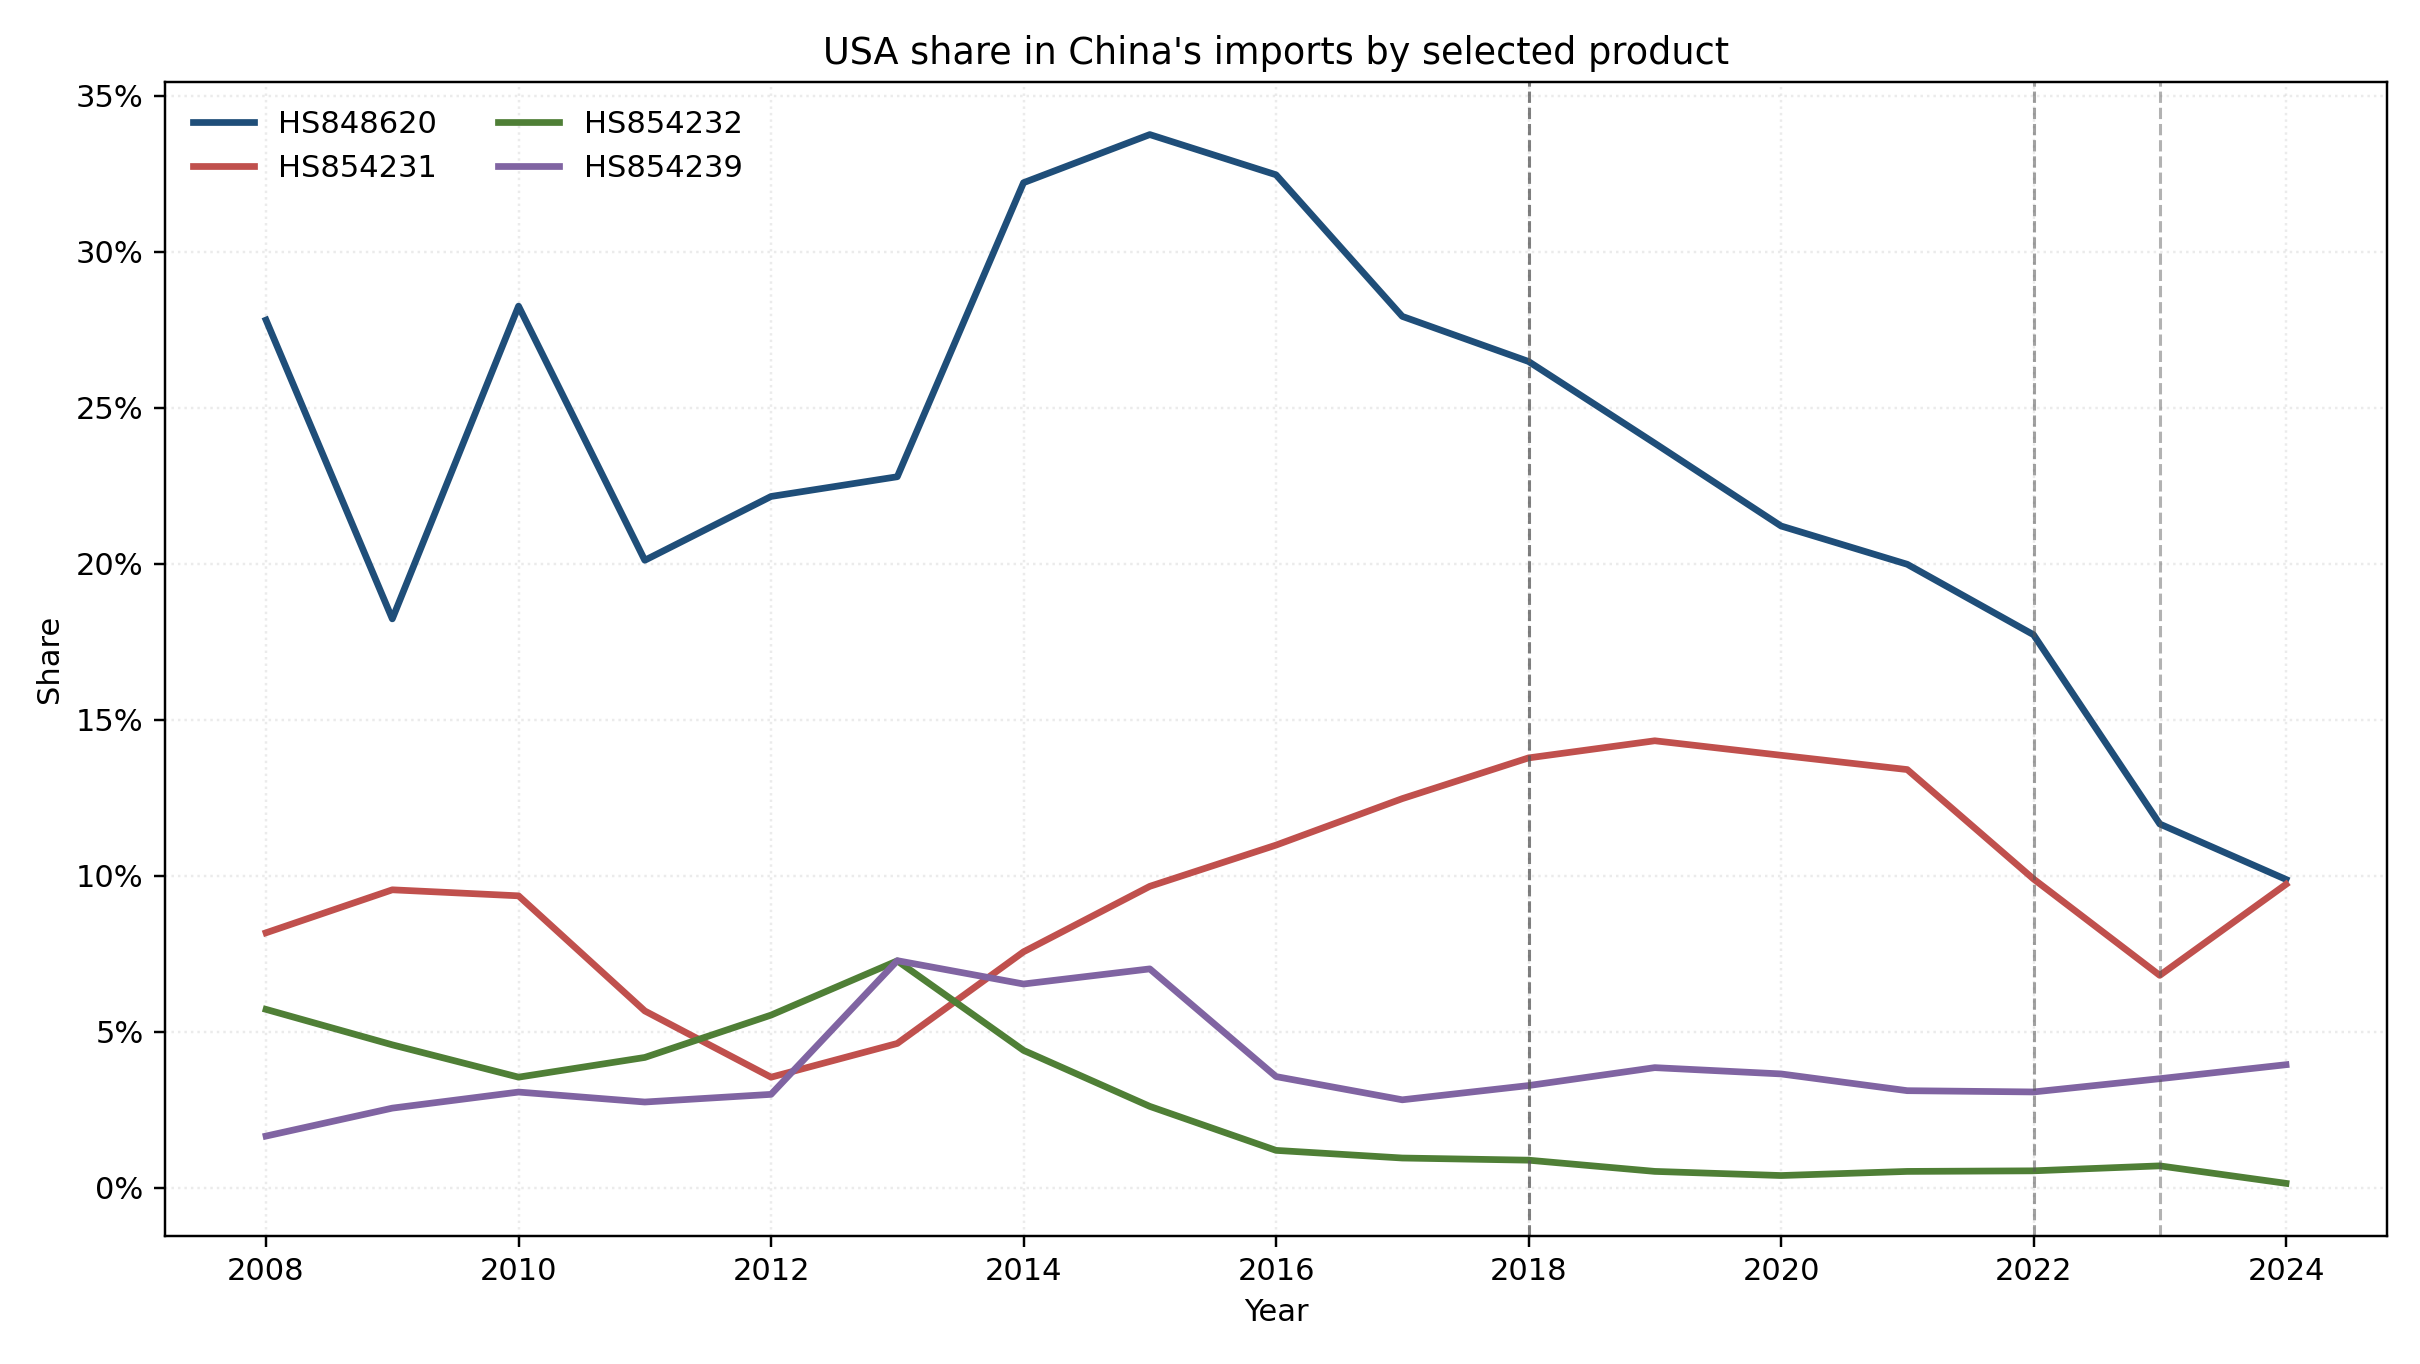
\includegraphics[width=0.92\textwidth]{usa_import_share_by_product_v02.png}
    \caption{美国来源进口份额变化}
    \label{fig:usa-share}
\end{figure}

2024 年主要来源国结构显示，设备类产品更多依赖日本、荷兰、新加坡和美国等设备强国；集成电路类产品则更多体现韩国、马来西亚、越南和 Other Asia, nes 等亚洲生产网络节点的作用。

\begin{figure}[H]
    \centering
    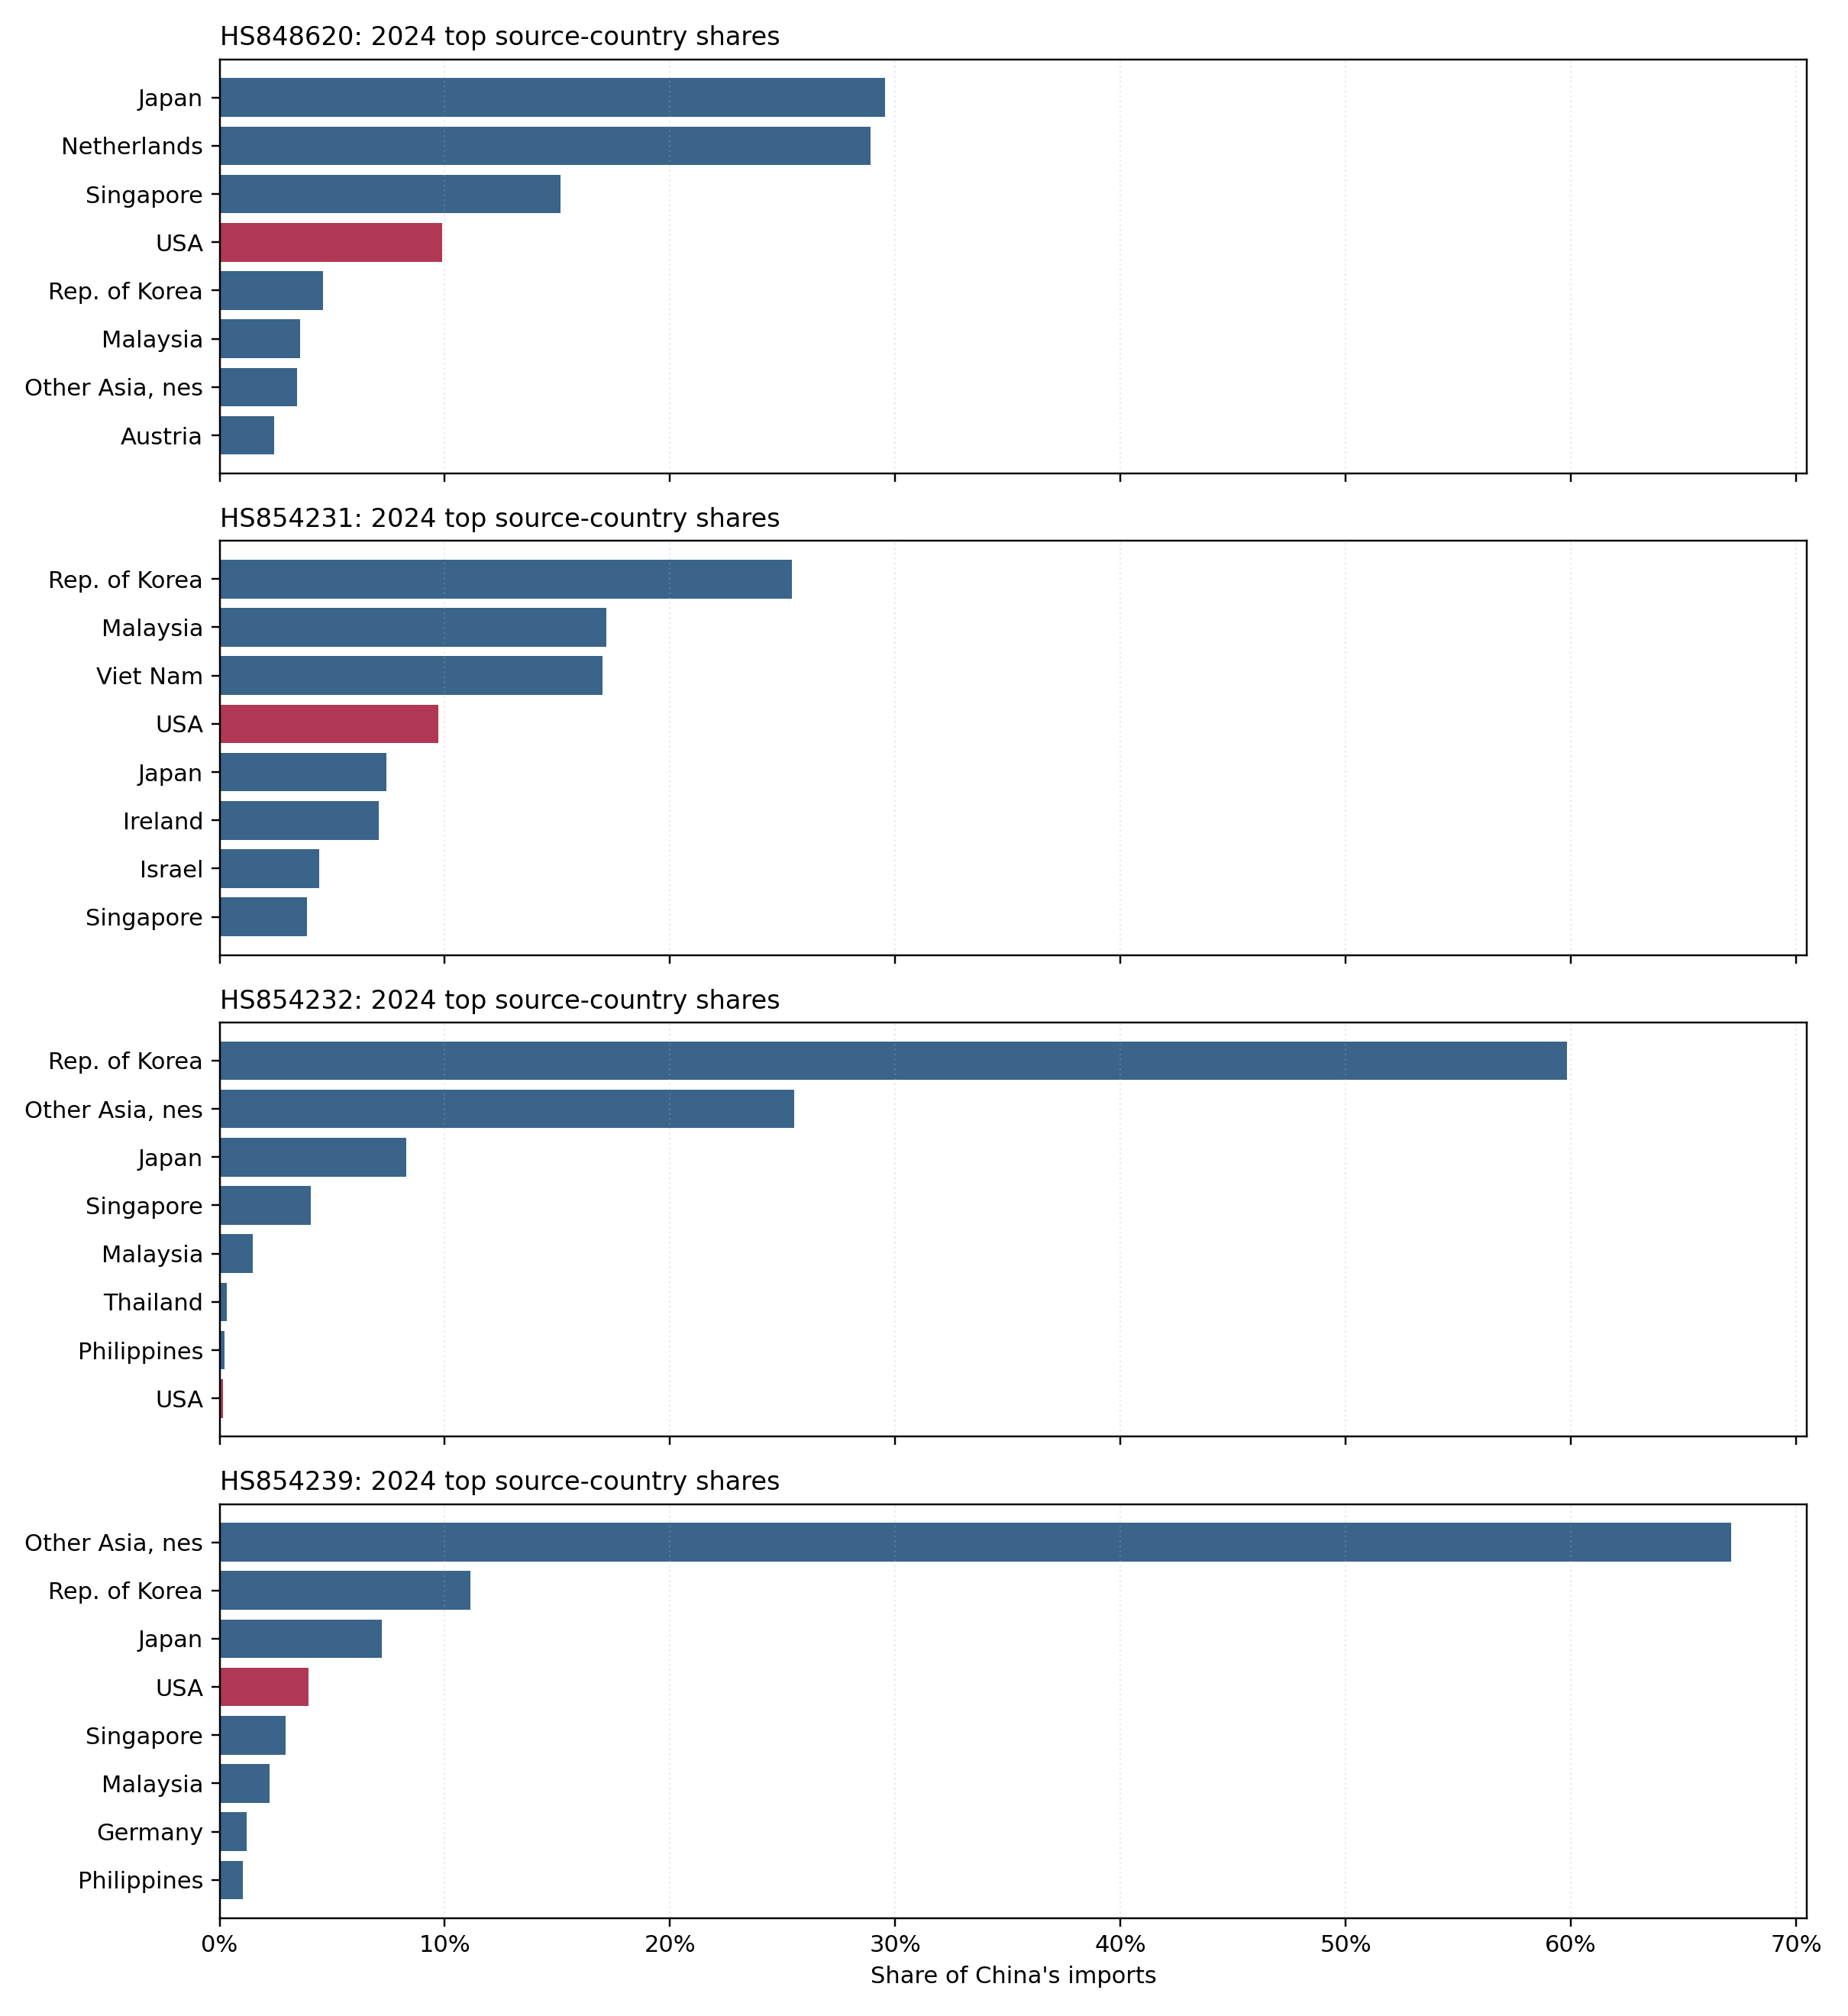
\includegraphics[width=0.92\textwidth]{top_2024_source_shares_by_product_v02.png}
    \caption{2024年主要来源国份额}
    \label{fig:top-sources}
\end{figure}

HHI 指标进一步说明，来源替代不等同于来源分散。部分产品在美国份额下降的同时，仍集中于少数主要来源国，因而需要综合指标评估供应链风险。

\begin{figure}[H]
    \centering
    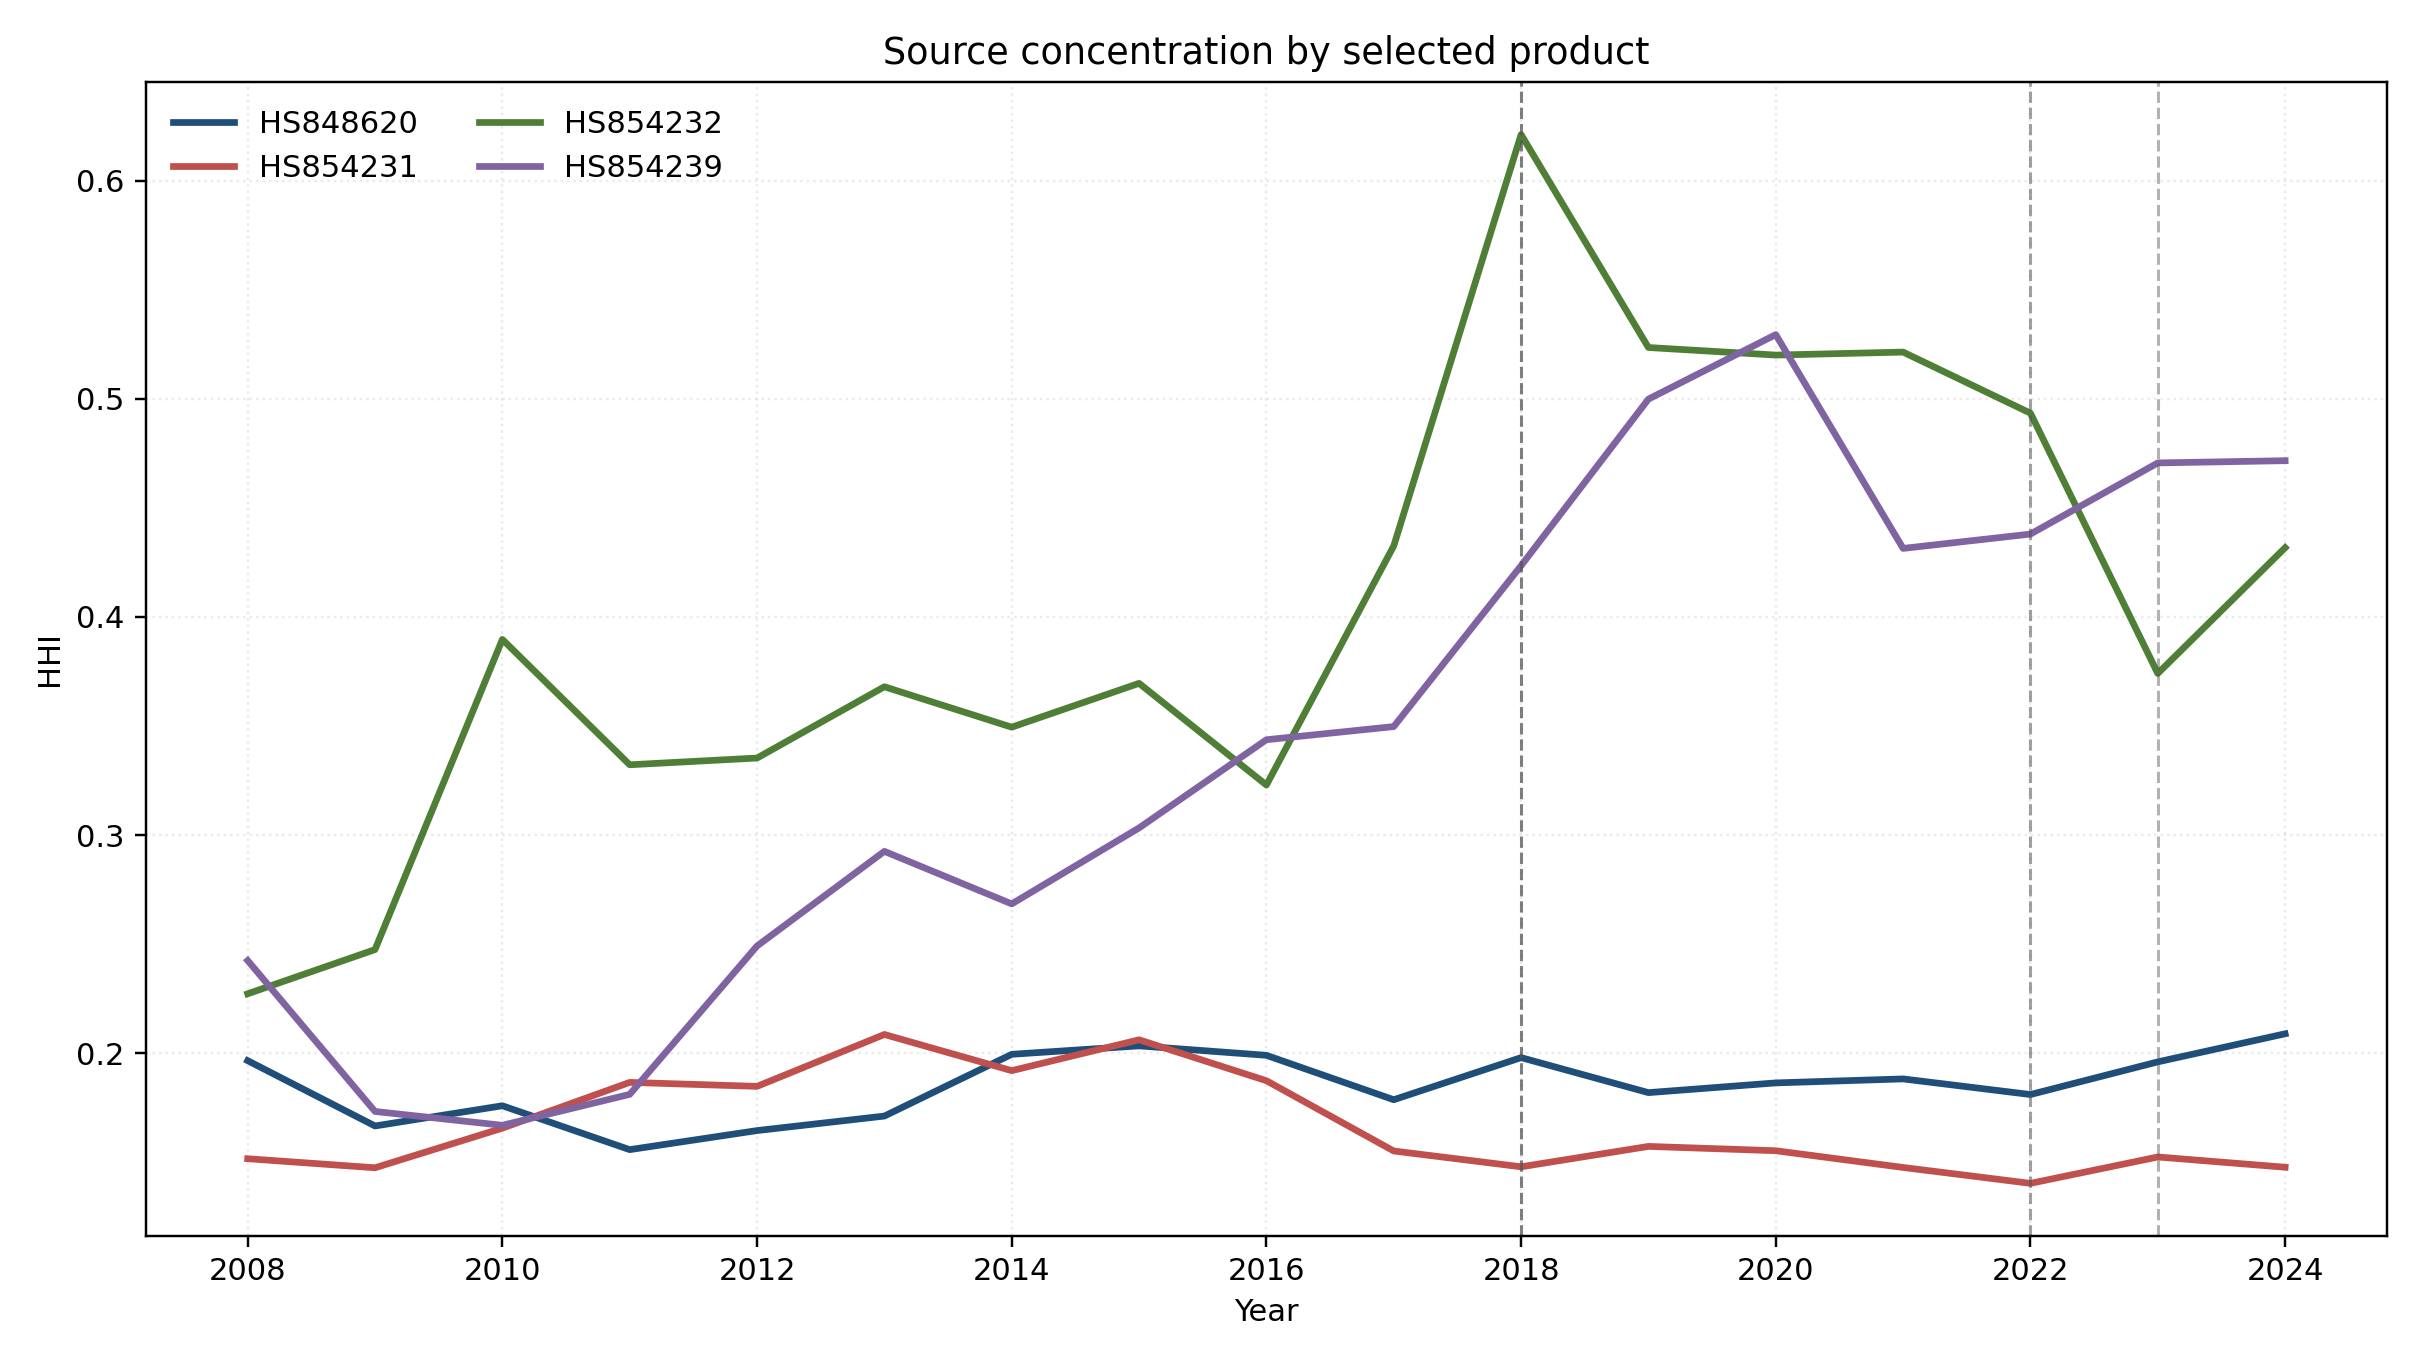
\includegraphics[width=0.92\textwidth]{source_hhi_by_product_v02.png}
    \caption{进口来源集中度 HHI}
    \label{fig:hhi}
\end{figure}

\section{半导体进口供应链风险指数构建}

为综合评价不同产品的进口来源结构风险，本文构建半导体进口供应链风险指数 SIRI。该指数按产品--年份计算，分值越高表示该产品在该年份的进口来源结构风险越高。SIRI 包含来源集中风险、政策暴露风险、替代不足风险和结构波动风险四个维度。

设 $s_{i,p,t}$ 为年份 $t$ 中国自来源国 $i$ 进口产品 $p$ 的份额。来源集中风险采用 HHI 衡量：
\[
C_{p,t}=\sum_i s_{i,p,t}^{2}.
\]
政策暴露风险使用美国来源份额衡量，即 $P_{p,t}=s_{US,p,t}$。替代不足风险使用非美国来源内部 HHI 衡量，若非美国来源越集中，则说明替代空间越弱。结构波动风险使用相邻年份来源份额的总变差距离：
\[
V_{p,t}=\frac{1}{2}\sum_i |s_{i,p,t}-s_{i,p,t-1}|.
\]
四个维度先在全部产品--年份样本内进行 0--1 标准化，再等权加总：
\[
SIRI_{p,t}=100\times(0.25C_{p,t}^{*}+0.25P_{p,t}^{*}+0.25A_{p,t}^{*}+0.25V_{p,t}^{*}).
\]
其中星号表示标准化后的指标。等权设定可以降低主观赋权影响。为检验结论稳健性，本文进一步将政策暴露风险权重提高至 0.40，其余三项权重设为 0.20。

\begin{figure}[H]
    \centering
    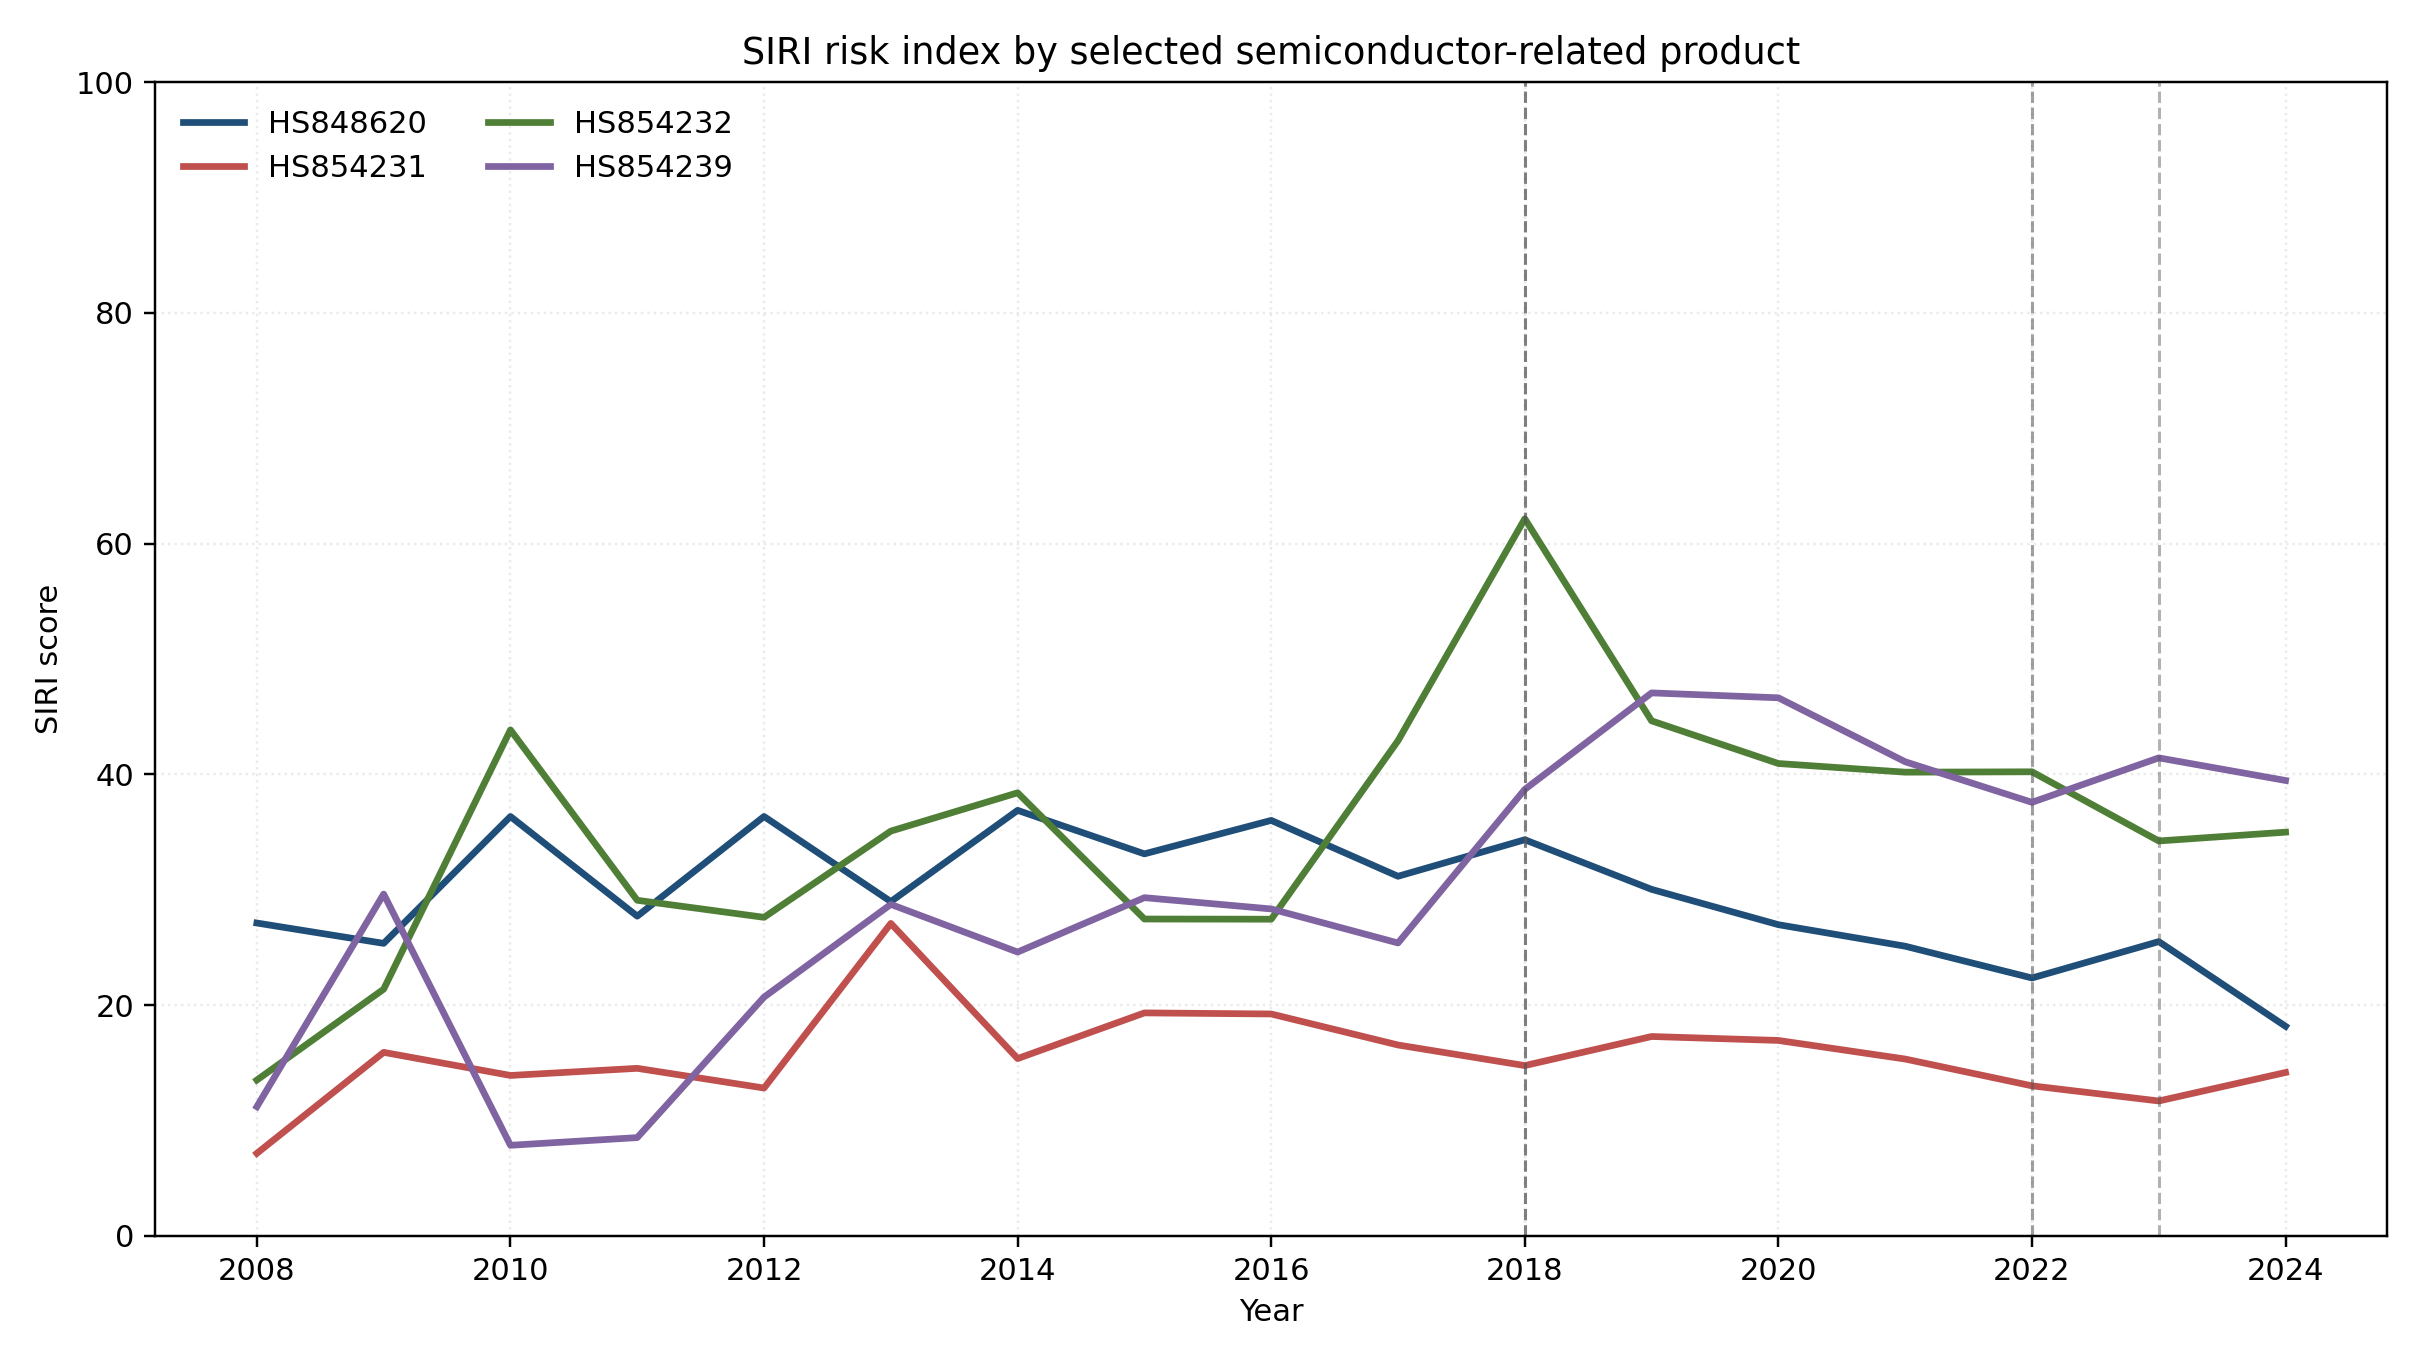
\includegraphics[width=0.92\textwidth]{siri_trend_by_product_v02.png}
    \caption{半导体相关产品 SIRI 风险指数变化趋势}
    \label{fig:siri-trend}
\end{figure}

表 \ref{tab:siri-ranking} 显示 2024 年 SIRI 排序。854239 和 854232 的综合风险相对更高，主要与来源集中和结构暴露有关。848620 虽然美国份额下降明显，但其 2024 年综合风险排序低于两类集成电路产品，说明设备类和集成电路类风险来源并不相同。

\begin{table}[H]
\centering
\caption{2024年 SIRI 风险指数排序}
\label{tab:siri-ranking}
\begin{tabular}{llrrr}
\toprule
排序 & HS6编码 & 基准SIRI & 政策暴露加权SIRI & 排序变化 \\
\midrule
1 & 854239 & 39.47 & 33.84 & 0 \\
2 & 854232 & 34.99 & 27.99 & 0 \\
3 & 848620 & 18.16 & 20.32 & 0 \\
4 & 854231 & 14.15 & 17.03 & 0 \\
\bottomrule
\end{tabular}
\end{table}


表 \ref{tab:siri-sensitivity} 给出权重敏感性检验。将政策暴露风险权重提高后，四类产品排序未发生变化，说明本文关于相对风险排序的结论不完全依赖单一权重设定。

\begin{table}[H]
\centering
\caption{SIRI 权重敏感性检验}
\label{tab:siri-sensitivity}
\begin{tabular}{lrrrrr}
\toprule
HS6编码 & 基准排序 & 政策加权排序 & 排序变化 & 基准得分 & 政策加权得分 \\
\midrule
854239 & 1 & 1 & 0 & 39.47 & 33.84 \\
854232 & 2 & 2 & 0 & 34.99 & 27.99 \\
848620 & 3 & 3 & 0 & 18.16 & 20.32 \\
854231 & 4 & 4 & 0 & 14.15 & 17.03 \\
\bottomrule
\end{tabular}
\end{table}


\section{政策节点下的统计检验与稳健性分析}

在描述统计和风险指数之外，本文使用固定效应回归考察政策节点后美国来源进口额的相对变化。基准模型设定为：
\[
\ln(Import_{i,p,t}+1)=\beta_1US_i\times Post2018_t+\beta_2US_i\times Post2022_t+\beta_3US_i\times Post2023_t+\alpha_i+\gamma_p+\delta_t+\varepsilon_{i,p,t}.
\]
其中 $\alpha_i$、$\gamma_p$ 和 $\delta_t$ 分别表示出口国固定效应、产品固定效应和年份固定效应。被解释变量首先采用进口额对数形式，并补充以进口份额为被解释变量的估计。

\begin{table}[H]
\centering
\caption{政策节点回归核心结果：进口额（OLS）与进口份额（PPML）}
\label{tab:regression}
\begin{tabular}{llrrc}
\toprule
 & 变量 & 系数 & 标准误 & p值 \\
\midrule
\multicolumn{5}{l}{\textit{列1：OLS，被解释变量 $\ln(Import+1)$}} \\
 & US$\times$Post2018 & 0.177 & 0.058 & 0.002 \\
 & US$\times$Post2022 & 0.026 & 0.048 & 0.589 \\
 & US$\times$Post2023 & -0.131 & 0.052 & 0.012 \\
\midrule
\multicolumn{5}{l}{\textit{列2：PPML，被解释变量 进口份额}} \\
 & US$\times$Post2018 & -0.053 & 0.074 & 0.478 \\
 & US$\times$Post2022 & -0.293 & 0.031 & $<$0.001 \\
 & US$\times$Post2023 & -0.320 & 0.062 & $<$0.001 \\
\bottomrule
\end{tabular}

\vspace{0.5em}
\begin{minipage}{0.92\linewidth}
\footnotesize
注：两列模型均包含出口国、产品和年份三重固定效应。列1使用按出口国聚类的稳健标准误，列2使用 PPML 估计，不报告传统 $R^2$。样本量 10\,608。
\end{minipage}
\end{table}


表 \ref{tab:regression} 显示，绝对进口额模型中 US$\times$Post2018、US$\times$Post2022 和 US$\times$Post2023 均不显著。份额型模型中三个交互项方向为负，但同样不显著。这一结果与描述统计并不矛盾：描述统计显示美国份额在部分产品中下降，但固定效应模型提醒我们，不能把这种结构变化简单解释为美国出口管制的严格因果效应。

稳健性检验包括改用反双曲正弦变换、剔除 2020--2021 年以及收窄到 2024 年前十来源国加美国的对照组。相关结果未改变核心判断：当前模型更适合支持“来源结构重组”和“美国份额承压”的经验事实，而不适合支持“美国对华出口额显著下降”的强因果结论。

\section{预测与预警扩展：基于贸易网络的 SIRI 风险预测}

\subsection{扩展目的}

前文分析主要回答两个问题：一是中国半导体相关产品进口来源结构如何变化，二是这些结构变化如何反映在 SIRI 供应链风险指数及其解释性回归中。作为进一步扩展，本节将问题推进到预测层面：如果已经观察到某一年产品的进口来源网络和风险特征，能否对下一年的 SIRI 风险水平形成可检验的预测。这一部分不替代前文的描述统计和回归主线，而是检验 SIRI 是否可以从事后评价指标扩展为下一年风险预测任务。

图 \ref{fig:v03-workflow} 概括了从 BACI 贸易数据到下一年 SIRI 预测评估的流程。

\begin{figure}[H]
    \centering
    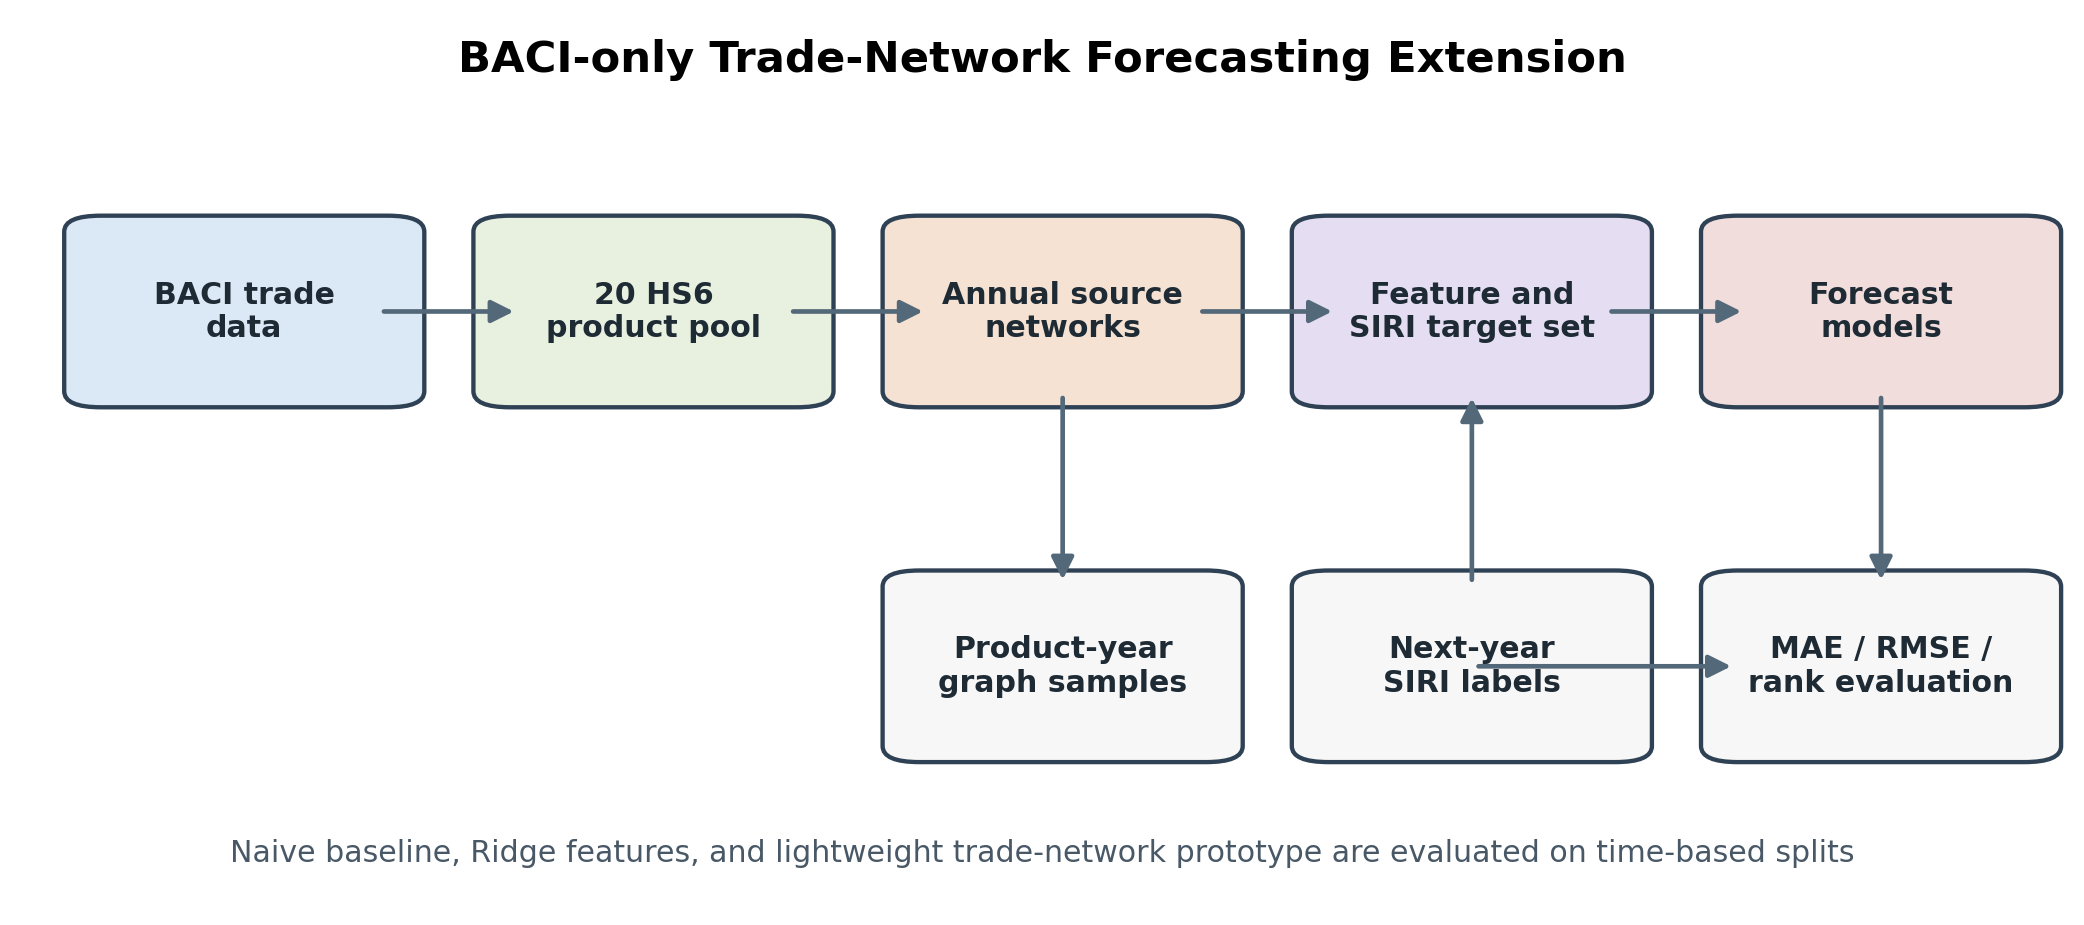
\includegraphics[width=0.98\textwidth]{v03_prediction_workflow.png}
    \caption{贸易网络预测扩展流程}
    \label{fig:v03-workflow}
\end{figure}

\subsection{数据扩展与图样本构造}

在数据与网络构造上，本节将产品范围从前文重点讨论的核心 4 个 HS6 产品扩展到 20 个半导体相关 HS6 产品。对每一个产品和每一个年份，本文构造一张中国进口来源网络：节点包括中国以及该年向中国出口该产品的来源国，边表示来源国向中国的出口关系，边权定义为该来源国在中国该产品年度进口额中的份额。因此，一个产品--年份对应一个年度图样本，图结构刻画的是进口来源集中度、来源国组合以及不同来源国在中国进口中的相对权重。样本规模与时间切分见表 \ref{tab:v03-overview}。

\begin{table}[H]
  \centering
  \caption{v0.3 贸易网络预测扩展样本概况}
  \label{tab:v03-overview}
  \begin{tabular}{lr}
    \toprule
    项目 & 数值 \\
    \midrule
    扩展产品数 & 20 \\
    年度图样本数 & 320 \\
    训练样本 & 240 \\
    验证样本 & 40 \\
    测试样本 & 40 \\
    GDELT 状态 & 未启用（BACI-only） \\
    \bottomrule
  \end{tabular}
\end{table}


\subsection{预测任务与模型比较}

预测设计采用一年期前瞻设定，即使用年份 $t$ 的贸易网络和风险特征预测 $t+1$ 年的产品级 SIRI。为避免把预测结果解释为政策冲击的因果识别，本文仅将其作为供应链风险预警的探索性任务，并在时间维度上划分训练、验证和测试样本。模型比较包括三类：Naive 基线使用上一年 SIRI 直接预测下一年 SIRI；Ridge 模型使用表格化风险特征进行线性正则化预测；贸易网络原型模型则利用图结构传播后的网络特征进行预测，用于检验年度进口来源图是否能提供额外的结构信息。这里的贸易网络原型对应轻量级 gcn\_numpy 原型，不等同于完整 GDELT-GCN 模型。测试集模型比较结果见表 \ref{tab:v03-metrics}。

\begin{table}[H]
  \centering
  \caption{v0.3 测试集预测指标比较}
  \label{tab:v03-metrics}
  \begin{tabular}{llrrrr}
    \toprule
    模型 & 样本范围 & MAE & RMSE & Spearman & 样本数 \\
    \midrule
    Naive & 全部20个产品 & 3.978 & 7.899 & 0.812 & 40 \\
    Naive & 核心4产品 & 1.667 & 2.117 & 0.881 & 8 \\
    Ridge & 全部20个产品 & 4.331 & 7.577 & 0.777 & 40 \\
    Ridge & 核心4产品 & 2.070 & 2.463 & 0.881 & 8 \\
    贸易网络原型 & 全部20个产品 & 61.179 & 263.756 & 0.601 & 40 \\
    贸易网络原型 & 核心4产品 & 1.974 & 2.444 & 0.857 & 8 \\
    \bottomrule
  \end{tabular}
  \caption*{注：当前 v0.3 结果为 BACI-only 贸易网络预测扩展，未接入真实 GDELT 新闻事件数据；“贸易网络原型”对应程序输出中的 gcn\_numpy 行，不代表完整 GDELT-GCN 模型。}
\end{table}


图 \ref{fig:v03-metrics-bar} 将测试集 MAE 和 RMSE 结果转化为分组柱状图。全部 20 个产品范围内，Naive 和 Ridge 的误差明显低于贸易网络原型；在核心 4 产品范围内，三类模型误差更接近，但复杂原型仍没有形成稳定优势。

\begin{figure}[H]
    \centering
    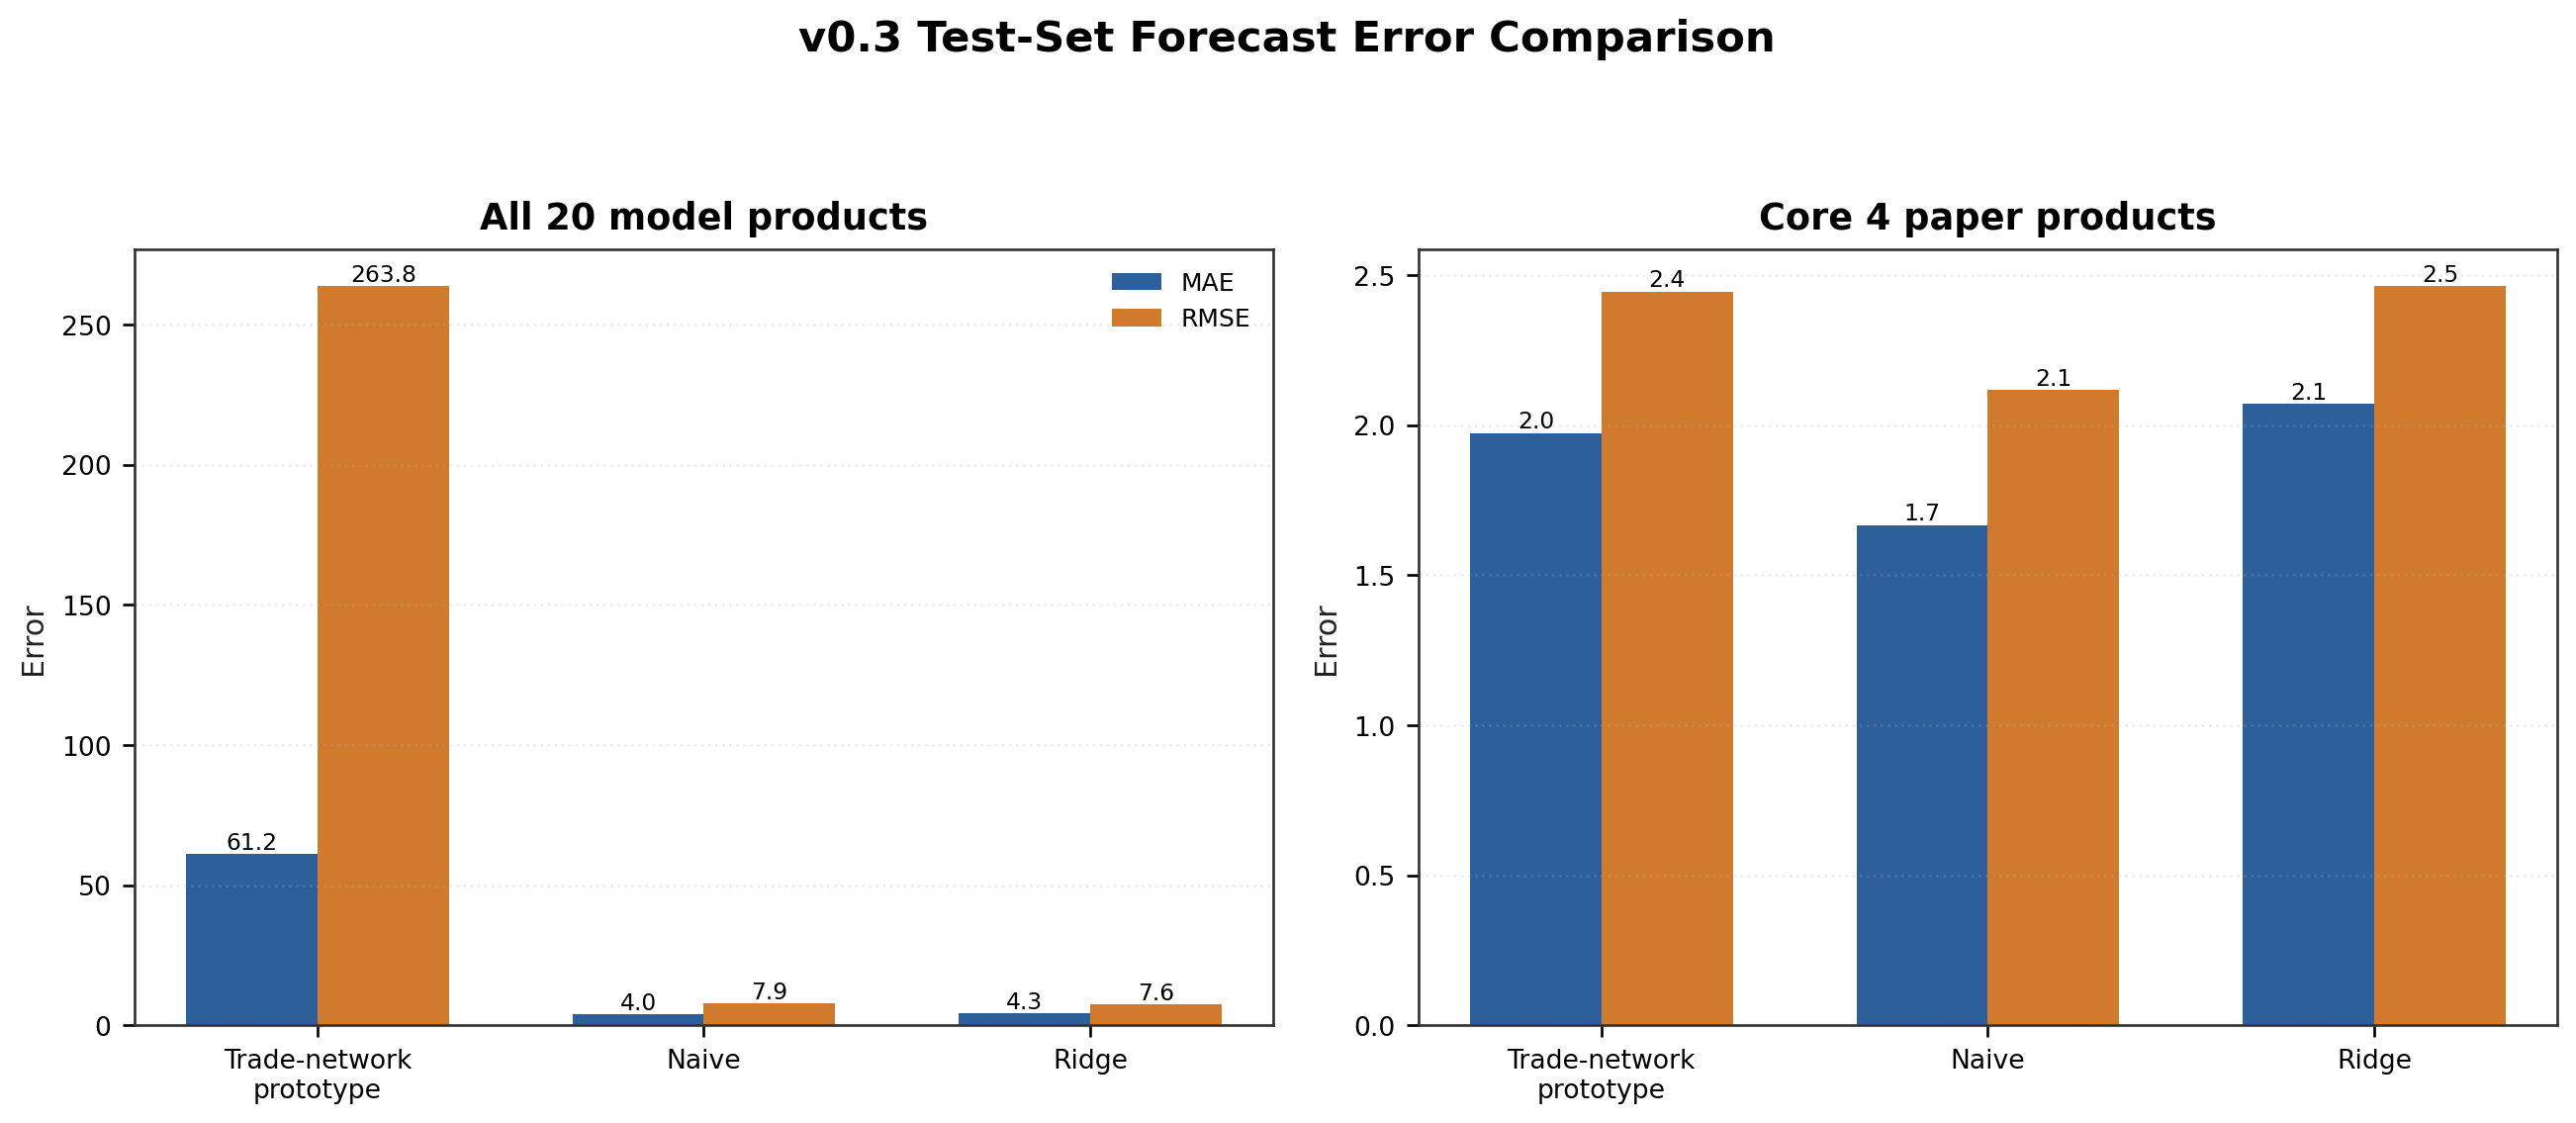
\includegraphics[width=0.96\textwidth]{prediction_metrics_bar.png}
    \caption{预测模型 MAE/RMSE 对比柱状图}
    \label{fig:v03-metrics-bar}
\end{figure}

\subsection{结果解读与预警价值}

结果显示，样本构造与评估流程表明，20 个产品、320 个年度图样本可以被组织为可复现的下一年 SIRI 预测任务。但从测试集指标看，在当前年度样本规模下，简单基线仍然具有较强竞争力，复杂贸易网络模型尚未体现出相对 Naive 或 Ridge 的稳定优势；其中贸易网络原型在全部 20 个产品上的误差明显偏大，说明该未约束原型在跨产品预测时仍不稳定。因此，贸易网络原型应被理解为探索性扩展，而不是对前文回归结论的强化证据。尤其需要说明的是，当前结果尚未启用真实 GDELT 新闻事件数据；本轮 BACI-only 扩展的主要价值在于建立产品--年份图样本、预测标签、基线比较和评估指标的统一框架，为后续接入 GDELT 新闻事件压力变量提供数据结构和评估框架。

\section{结论与政策建议}

本文基于 BACI HS07 2008--2024 年中国进口贸易数据，研究四类半导体相关产品的进口来源结构演化，并构建 SIRI 风险指数评价供应链风险。主要结论如下。

第一，中国半导体相关产品进口来源结构在 2018 年后出现明显重组。848620、854231 和 854232 的美国进口份额下降，854239 则小幅上升，说明不能将所有半导体相关产品概括为同一种变化方向。

第二，不同产品的风险暴露存在显著异质性。设备类产品的替代来源更多集中于日本、荷兰、新加坡等设备强国；集成电路类产品则更多体现亚洲生产网络内部调整。SIRI 指数显示，2024 年 854239 和 854232 的综合风险相对更高。

第三，固定效应回归结果不支持将来源结构变化简单归因为美国出口管制的严格因果效应。更稳妥的表述是：政策冲击背景下，中国半导体相关产品进口来源结构发生重组，美国份额在部分产品中承压，但绝对进口额变化仍受到产业周期、需求扩张和第三方产能变化等因素共同影响。

基于以上发现，本文提出三点建议。其一，对设备类和集成电路类产品采取差异化风险监测，不宜用单一产品结论推断整体半导体供应链。其二，持续跟踪来源集中度和替代来源结构，尤其关注高 SIRI 产品的主要来源国集中风险。其三，将风险指数作为动态监测工具，与企业层面供应链信息和更高频贸易数据结合，提高关键产品进口安全预警能力。


% ============ 参考文献 ============
\clearpage
\phantomsection
\addcontentsline{toc}{section}{参考文献}
\bibliographystyle{unsrtnat}
\bibliography{references}

% ============ 附录 ============
\clearpage
\appendix
\phantomsection
\addcontentsline{toc}{section}{附录}
\section*{\heiti\zihao{4} 附\quad 录}
\subsection{复现说明}

\subsubsection{运行命令}

主要复现命令如下：
\begin{verbatim}
.venv/bin/python scripts/run_analysis.py
.venv/bin/python scripts/run_gcn_analysis.py --baci-only
\end{verbatim}
若需从原始数据完整复现，需要将 BACI HS07 V202601 原始数据目录放置于项目根目录下的 \texttt{BACI\_HS07\_V202601/}。

\subsubsection{GDELT 数据接口预留}

本文预测扩展结果使用 BACI-only 模式生成；若需启用 GDELT 新闻事件压力变量，可使用如下命令：
\begin{verbatim}
.venv/bin/python scripts/run_gcn_analysis.py \
  --gdelt-events data/gdelt/prefiltered_events.csv
\end{verbatim}
该 CSV 至少需要包含以下字段：
\begin{itemize}
  \item \texttt{SQLDATE}
  \item \texttt{Actor1CountryCode}、\texttt{Actor2CountryCode}
  \item \texttt{GoldsteinScale}、\texttt{NumMentions}、\texttt{AvgTone}
\end{itemize}

\subsection{变量说明}

\begin{longtable}{@{}>{\raggedright\arraybackslash}p{0.43\textwidth}>{\raggedright\arraybackslash}p{0.53\textwidth}@{}}
\toprule
变量 & 含义 \\
\midrule
\endhead
\texttt{import\_value\_kusd} & 中国自某来源国进口某产品的年度金额，单位为千美元 \\
\texttt{import\_share} & 来源国进口额占产品--年份总进口额的比例 \\
\texttt{US} & 来源国是否为美国 \\
\texttt{Post2018} & 年份是否不早于 2018 年 \\
\texttt{Post2022} & 年份是否不早于 2022 年 \\
\texttt{Post2023} & 年份是否不早于 2023 年 \\
\texttt{siri\_score} & 基准 SIRI 风险指数得分 \\
\texttt{siri\_score\_policy\_weighted} & 提高政策暴露权重后的 SIRI 得分 \\
\bottomrule
\end{longtable}

\subsection{AI 工具使用说明}

本文写作和代码整理过程中使用 AI 工具辅助结构设计、代码实现建议、LaTeX 排版和文字润色。数据来源、模型设定、结果解释和最终结论由参赛队审核确认。具体使用记录见表 \ref{tab:ai-usage}。

\begin{table}[H]
  \centering
  \caption{AI 工具使用记录}
  \label{tab:ai-usage}
  \begin{tabular}{@{}p{1.8cm}p{1.2cm}p{1.6cm}p{4.2cm}p{4.2cm}@{}}
    \toprule
    日期 & 工具 & 使用阶段 & 具体任务 & 人工审核 \\
    \midrule
    2026-04-28 & Codex & 选题设计 & 提供论文结构与 SIRI 指标公式备选方案，由参赛队筛选确认 & 参赛队审阅后确认研究边界与最终表述 \\
    2026-04-28 & Codex & 代码辅助 & 协助实现 SIRI 指数计算、图表输出、验证检查和单元测试 & 参赛队核对代码逻辑、输出表格和论文表述 \\
    2026-04-28 & Codex & LaTeX 排版 & 协助搭建论文模板、章节结构和表格格式 & 参赛队逐章审阅并修改正文表述 \\
    \bottomrule
  \end{tabular}
\end{table}


% ============ 致谢 ============
\clearpage
\phantomsection
\addcontentsline{toc}{section}{致谢}
\begin{center}
{\heiti\zihao{4} 致\quad 谢}
\end{center}
\hspace{2em}衷心感谢指导教师李晓花老师在本次统计建模大赛全程中给予的悉心指导与及时帮助。李老师在选题方向、排版规范和公式选择等关键环节提出了许多宝贵建议，使我们在研究思路和论文撰写上受益匪浅。

感谢队友于重阳、龚旭和余博的密切协作。余博承担了数据处理与图表绘制工作，龚旭负责确定选题、排版校对与论文架构设计，于重阳负责论文文稿的编写与修改。三人各司其职、相互配合，共同完成了本次研究。

\begin{flushright}
2026 年 5 月 2 日
\end{flushright}

\end{document}
